\documentclass[journal]{IEEEtran}
\usepackage[T1]{fontenc}
\usepackage{amsmath,amssymb}
\usepackage{graphicx}
\usepackage{booktabs}
\usepackage{multirow}
\usepackage{array}
\usepackage{xcolor}
\usepackage{algorithm}
\usepackage[noend]{algpseudocode}
\usepackage{tikz}
\usetikzlibrary{arrows.meta,positioning,calc}
\usepackage{cite}
\usepackage{url}
\usepackage[hidelinks]{hyperref}
\graphicspath{{figures/}}

\newcommand{\dc}{$\Delta$Context}
\newcommand{\todo}[1]{\textcolor{red}{[#1]}}
\renewcommand{\algorithmicrequire}{\textbf{Input:}}
\renewcommand{\algorithmicensure}{\textbf{Output:}}

\begin{document}

\title{\dc{}: Delayed-Commitment Online Topic Segmentation for Topic-Indexed Conversational Memory}

\author{Pravin~Raj and \todo{Co-author / supervisor names}%
\thanks{\todo{Department, institution, city, country; e-mail addresses.}}%
\thanks{Code, configurations and per-question outputs: \todo{repository URL}.}}

\markboth{\todo{Journal name}}{Raj \MakeLowercase{\textit{et al.}}: \dc{}: Delayed-Commitment Online Topic Segmentation}

\maketitle

\begin{abstract}
Chat assistants that persist across sessions accumulate histories far longer
than their context windows, so every query requires choosing which past turns
the model sees. Storing the history as topic segments makes earlier topics
cheap to revisit and search, but offline segmenters redraw boundaries as the
chat grows, and online rules cut at the first semantic jump. This paper
proposes \dc{}, an online segmenter that delays each boundary decision by a few
turns, compares the open topic with the turns that follow, and commits a
boundary only at a local maximum of semantic distance, never revising it. The
segments index a topic-first store. On LongMemEval-S histories of about 490
turns, \dc{} is the most accurate segmenter compared (Pk 0.058 against 0.069
for the best offline method) with zero boundary revisions, against about 17
per 100 turns for offline methods. Its store retrieves as well as a
true-session store, and its answers are statistically tied with a full scan's
while searching 17\% of the turns.
\end{abstract}

\begin{IEEEkeywords}
Conversational memory, dialogue topic segmentation, online segmentation,
retrieval-augmented generation, large language models, context management.
\end{IEEEkeywords}

% =====================================================================
\section{Introduction}

\IEEEPARstart{D}{ialogue} systems built on large language models (LLMs) are
moving from single-session tools to long-lived assistants
\cite{ni2023survey,wang2024agents}. An assistant that remembers earlier
sessions must manage a memory that grows without bound, and memory has become
a central design question for LLM-based agents \cite{zhang2025memory}. Simply
enlarging the prompt does not solve it: attention cost grows with input length
\cite{tay2022efficient}, models use information in the middle of long inputs
unreliably \cite{liu2024lost}, and irrelevant or missing context is a known
source of hallucination \cite{huang2025hallucination}.

Practical systems therefore select, for each query, a small set of past turns
under a token budget. Retrieval-augmented generation (RAG) embeds stored text
and fetches the passages most similar to the query
\cite{wu2026rag,zhao2024dense}, usually from a vector index
\cite{pan2024vectordb}; summarisation compresses older turns into a running
memory \cite{wang2025recursive}; and memory architectures such as MemoryBank
and MemGPT combine storage with update and paging rules
\cite{zhong2024memorybank,packer2023memgpt}. The LongMemEval benchmark showed
that long-context LLMs lose about 30\% accuracy on chat histories of
$\sim$115K tokens and identified the granularity at which history is stored as
a key memory design choice \cite{wu2025longmemeval}.

A natural unit of storage for a conversation is the \emph{topic}. Topic-aware
modelling improves dialogue comprehension and response selection
\cite{ma2024topicaware} and response generation \cite{sun2022hierarchical},
dialogue topic segmentation remains an active research problem
\cite{xu2025umlf}, and retrieval quality depends on how text is chunked before
indexing \cite{lavarec2026chunking}. If a chat history is stored as topic
segments as it arrives, an assistant can first find the right topic and then
search only inside it, which is cheaper than scanning every turn, and returning
to an earlier topic means reopening one stored unit rather than re-reading the
history.

\textbf{Problem statement.} Building such a store requires a segmenter that
works on a stream. The most accurate unsupervised segmenters are offline: they
score every gap of a finished dialogue and then choose boundaries. On a growing
chat they must be re-run, and each re-run can move or delete boundaries that
already index the store. The simplest online rule, cutting where two
consecutive turns differ, decides from a single pair of turns and is noisy. The
question this paper addresses is whether an online segmenter that never revises
a boundary can match offline segmenters, and whether a store indexed by it
retrieves as well as one built from the true topic structure.

\textbf{Objective.} To design an online, training-free topic segmenter whose
boundaries are final when made, and to use it as the index of a topic-first
conversational memory that keeps retrieval and answer quality at a fraction of
the search cost of a full scan.

\textbf{Contributions.}
\begin{enumerate}
\item \dc{}, a \emph{delayed-commitment} online segmenter. Each gap between
turns is scored after $L$ further turns against the recent part of the open
topic, and a boundary is committed only at a local maximum above a threshold.
Boundaries are never revised, the decision delay is a constant $L{+}1$ turns,
and no training is needed.
\item A topic-first conversational store indexed by these segments, with
two-stage retrieval (topic centroids, then turns) under a token budget.
\item A controlled evaluation on four datasets with dev-only tuning, a single
test pass and Holm-corrected paired bootstrap tests. It includes an
equal-selection protocol, streaming stability, retrieval, scaling to
$\sim$20K turns and end-to-end question answering.
\item Evidence that \dc{} is the most accurate segmenter on long chat
histories, including against offline TextTiling (Pk 0.058 vs.\ 0.069,
$p<10^{-4}$), and the best online method on all four datasets; that it makes
zero boundary revisions; and that its store matches a true-session store while
answering as well as a full scan from 17.1\% of the comparisons.
\end{enumerate}

\textbf{Organisation.} Section~\ref{sec:lit} reviews related work and states
the identified gap. Section~\ref{sec:method} presents the four phases of
\dc{}. Section~\ref{sec:results} gives the experimental setup, datasets and
results. Section~\ref{sec:comp} compares \dc{} with existing works on several
metrics, and Section~\ref{sec:concl} concludes.

% =====================================================================
\section{Literature Review}
\label{sec:lit}

\subsection{Memory for long-running conversations}
MemoryBank \cite{zhong2024memorybank} stores memories with summaries and an
Ebbinghaus-style forgetting rule; MemGPT \cite{packer2023memgpt} lets the LLM
page information between the prompt and external storage; Wang et al.\
\cite{wang2025recursive} recursively rewrite a summary memory; and LongMemEval
\cite{wu2025longmemeval} proposes session decomposition, fact-augmented keys
and time-aware query expansion. None derives topic units from the stream: they
store fixed units (turns, rounds, sessions) or LLM-written summaries, which
cost an LLM call per update.

\subsection{Dialogue topic segmentation}
TextTiling \cite{hearst1997texttiling} places boundaries at depth-score minima
of a similarity curve over a complete text and is still the decoding step of
neural methods such as CSM \cite{xing2021csm}, which trains a BERT coherence
scorer on automatically built utterance pairs. DialSTART
\cite{gao2023dialstart} learns topic-aware utterance representations by
contrastive learning, and UMLF \cite{xu2025umlf} jointly learns discourse
parsing and topic segmentation without labels, reporting the best unsupervised
results on DialSeg711 and TIAGE. SuperDialseg \cite{jiang2023superdialseg}
shows that supervised models are strong in domain, Ma et al.\
\cite{ma2024topicaware} use unsupervised topic blocks for comprehension, and
Nouar and Belhadef \cite{nouar2026boundary} audit why a supervised segmenter
places its boundaries. All of these segment a complete, short dialogue offline;
none addresses a stream whose boundaries index a store.

\subsection{Chunking and label-free semantic structure}
Semantic chunking \cite{langchain2024semantic} splits text where consecutive
embeddings differ by more than a percentile of all distances, so it needs the
whole text. Lavarec and Du \cite{lavarec2026chunking} compare fixed-size,
recursive, semantic and LLM-based chunking for RAG and find structure-preserving
recursive chunking best, but a chat log lacks the headings and paragraphs it
relies on. More broadly, label-free use of distributional and contextual
semantics has proven effective for building structure from text: weighted
distributional models for named-entity recognition \cite{veena2023agroner}, bootstrapped
syntax--semantics relation extraction for knowledge-graph construction
\cite{veena2023relation}, BERT-strengthened guided topic models for aspect
extraction \cite{venugopalan2022guidedlda}, and topic- and concept-guided
summarisation with transformers \cite{gurusamy2023summarization}. \dc{}
applies the same label-free principle to the geometry of a conversation's turn
embeddings. Table~\ref{tab:lit} summarises ten recent works most similar to
ours.

\begin{table*}[t]
\centering
\caption{Ten recent related works: method, advantage and drawback with respect to an online topic-indexed conversational memory.}
\label{tab:lit}
\footnotesize
\renewcommand{\arraystretch}{1.1}
\setlength{\tabcolsep}{4pt}
\begin{tabular}{@{}p{2.5cm}p{0.6cm}p{4.3cm}p{3.9cm}p{5.4cm}@{}}
\toprule
Work & Year & Algorithm & Advantage & Drawback for our setting \\
\midrule
MemoryBank \cite{zhong2024memorybank} & 2024 & Memory store with summaries, Ebbinghaus-style forgetting, dense retrieval & Persistent, user-adaptive memory & Flat store of fixed memory units; no topic structure \\
MemGPT \cite{packer2023memgpt} & 2023 & LLM-managed paging between prompt and external storage & Unbounded virtual context & Every memory operation is an LLM call; no topic structure \\
Recursive summarisation \cite{wang2025recursive} & 2025 & LLM rewrites memory from previous memory and new turns & Compact memory, complements long-context LLMs & Lossy; errors accumulate; verbatim evidence is lost \\
LongMemEval \cite{wu2025longmemeval} & 2025 & Benchmark; session decomposition, key expansion, time-aware queries & Systematic memory design study on 115K-token histories & Relies on given session boundaries; flat index over all rounds \\
DialSTART \cite{gao2023dialstart} & 2023 & Topic-aware contrastive learning of utterance representations & Strong unsupervised accuracy & Needs in-domain training; offline, boundaries change on re-run \\
SuperDialseg \cite{jiang2023superdialseg} & 2023 & 9,478 labelled dialogues; 18-model benchmark & Supervised models strong in domain & Needs labels; short dialogues; no streaming setting \\
Topic-aware comprehension \cite{ma2024topicaware} & 2024 & Unsupervised topic blocks + dual-attention matching (TADAM) & Segments aid comprehension and response selection & Segments a finished passage; no store or retrieval cost \\
UMLF \cite{xu2025umlf} & 2025 & Mutual learning of discourse parsing and topic segmentation & Best unsupervised Pk on DialSeg711 and TIAGE & Several large encoders; offline decoding \\
Chunking for RAG \cite{lavarec2026chunking} & 2026 & Fixed, recursive, semantic and LLM chunking compared for RAG & Shows chunking choice changes retrieval and answers & Static documents; recursive splitting needs document structure \\
Boundary explainability \cite{nouar2026boundary} & 2026 & Perturbation-based explanation of a supervised hierarchical segmenter & Audits why boundaries are predicted & Supervised, offline; does not improve segmentation \\
\bottomrule
\end{tabular}
\end{table*}

\subsection{Identified problem}
The review exposes four gaps. (i) Conversational memories store fixed units or
summaries, not topics found online. (ii) Accurate dialogue segmenters are
offline: on a growing chat they must be re-run, which revises boundaries that
already index stored data. (iii) Online rules decide from a single pair of
turns. (iv) No prior work measures whether online topic segmentation is good
enough to index a conversational memory, at scale and end to end. \dc{}
targets this combination: online, revision-free, training-free segmentation
evaluated as the index of a memory.

% =====================================================================
\section{Proposed Work}
\label{sec:method}

\subsection{Overview}
\dc{} runs in four phases (Fig.~\ref{fig:arch}). Phases 1--3 run once per
incoming turn and maintain the store; Phase 4 runs once per query. A
conversation is a stream of turns $u_1,u_2,\dots$; turn $t$ has a unit-norm
embedding $e_t\in\mathbb{R}^d$. Gap $g$ lies between turns $g$ and $g{+}1$,
and a boundary at gap $g$ starts a new topic at turn $g{+}1$. The open topic
starts at turn $a$.

\begin{figure*}[t]
\centering
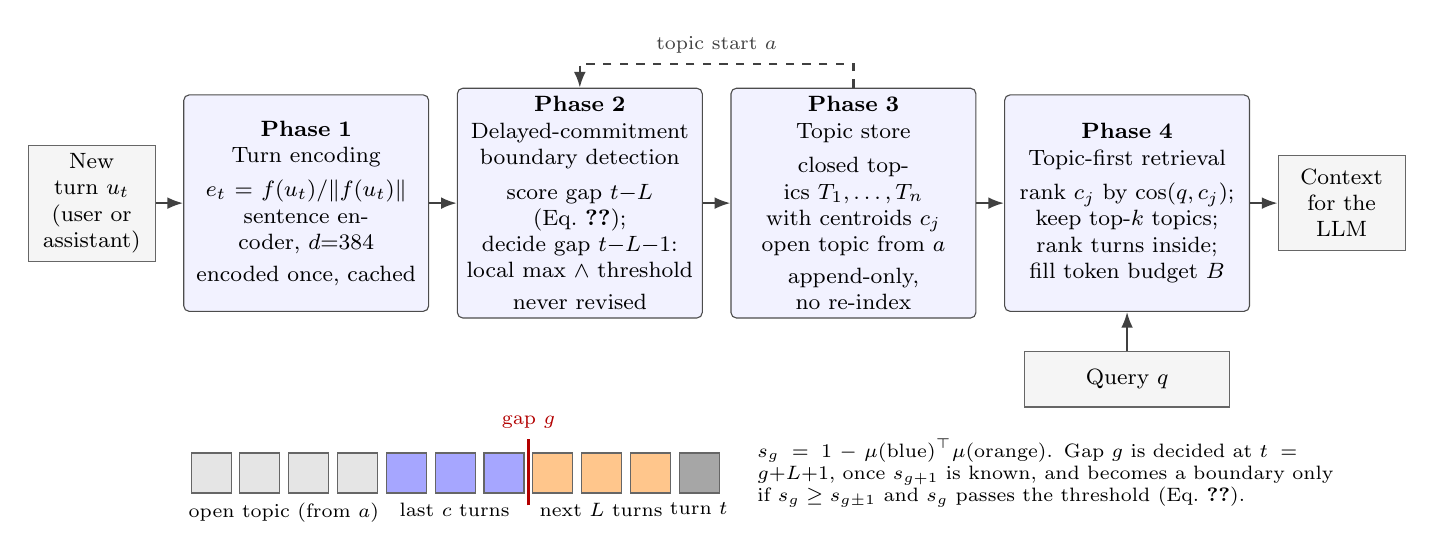
\begin{tikzpicture}[
  node distance=3.5mm,
  phase/.style={draw=black!70, rounded corners=2pt, fill=blue!5, align=center,
                text width=2.9cm, minimum height=2.75cm, font=\footnotesize, inner sep=3pt},
  io/.style={draw=black!60, fill=black!4, align=center, text width=1.4cm,
             minimum height=1.2cm, font=\footnotesize, inner sep=3pt},
  arr/.style={-{Latex[length=2mm]}, thick, black!75}]
\node[io] (in) {New turn $u_t$\\(user or\\assistant)};
\node[phase, right=of in] (p1) {\textbf{Phase 1}\\Turn encoding\\[3pt]
  $e_t = f(u_t)/\lVert f(u_t)\rVert$\\sentence encoder, $d{=}384$\\[2pt]
  encoded once, cached};
\node[phase, right=of p1] (p2) {\textbf{Phase 2}\\Delayed-commitment\\boundary detection\\[3pt]
  score gap $t{-}L$ (Eq.~\ref{eq:score});\\decide gap $t{-}L{-}1$:\\
  local max $\wedge$ threshold\\[2pt] never revised};
\node[phase, right=of p2] (p3) {\textbf{Phase 3}\\Topic store\\[3pt]
  closed topics $T_1,\dots,T_n$\\with centroids $c_j$\\open topic from $a$\\[2pt]
  append-only, no re-index};
\node[phase, right=of p3] (p4) {\textbf{Phase 4}\\Topic-first retrieval\\[3pt]
  rank $c_j$ by $\cos(q,c_j)$;\\keep top-$k$ topics;\\rank turns inside;\\
  fill token budget $B$};
\node[io, right=of p4] (out) {Context\\for the LLM};
\node[io, below=5mm of p4, text width=2.4cm, minimum height=0.7cm] (q) {Query $q$};
\draw[arr] (in) -- (p1);
\draw[arr] (p1) -- (p2);
\draw[arr] (p2) -- (p3);
\draw[arr] (p3) -- (p4);
\draw[arr] (p4) -- (out);
\draw[arr] (q) -- (p4);
\draw[arr, dashed] (p3.north) -- ++(0,3mm) -| node[pos=0.25, above, font=\scriptsize]{topic start $a$} (p2.north);
% ---- delayed commitment illustration ----
\begin{scope}[shift={($(p1.south west)+(0.1,-2.3)$)}, x=0.62cm, y=0.62cm]
  \foreach \i in {0,...,10} {
    \ifnum\i<4 \fill[black!10] (\i,0) rectangle ++(0.82,0.82);\fi
    \ifnum\i>3 \ifnum\i<7 \fill[blue!35] (\i,0) rectangle ++(0.82,0.82);\fi\fi
    \ifnum\i>6 \ifnum\i<10 \fill[orange!45] (\i,0) rectangle ++(0.82,0.82);\fi\fi
    \ifnum\i=10 \fill[black!35] (\i,0) rectangle ++(0.82,0.82);\fi
    \draw[black!60] (\i,0) rectangle ++(0.82,0.82);
  }
  \draw[very thick, red!70!black] (6.91,-0.25) -- (6.91,1.1) node[above, font=\scriptsize]{gap $g$};
  \node[font=\scriptsize, below] at (1.9,0) {open topic (from $a$)};
  \node[font=\scriptsize, below] at (5.4,0) {last $c$ turns};
  \node[font=\scriptsize, below] at (8.4,0) {next $L$ turns};
  \node[font=\scriptsize, below] at (10.4,0) {turn $t$};
  \node[font=\scriptsize, anchor=west, align=left, text width=7.4cm] at (11.4,0.41)
    {$s_g = 1-\mu(\text{blue})^{\top}\mu(\text{orange})$. Gap $g$ is decided at
     $t=g{+}L{+}1$, once $s_{g+1}$ is known, and becomes a boundary only if
     $s_g\ge s_{g\pm1}$ and $s_g$ passes the threshold (Eq.~\ref{eq:rule}).};
\end{scope}
\end{tikzpicture}
\caption{Architecture of \dc{}: four phases, with Phases 1--3 run per turn and
Phase 4 per query. The strip below illustrates delayed commitment with
$c{=}L{=}3$: a gap is scored when $L$ later turns exist and decided one turn
later, after which the decision is final.}
\label{fig:arch}
\end{figure*}

\subsection{Phase 1: turn encoding}
Each turn is prefixed with its speaker role and encoded by a sentence encoder
$f$ (all-MiniLM-L6-v2, $d{=}384$ \cite{reimers2019sbert}), then normalised:
$e_t=f(u_t)/\lVert f(u_t)\rVert$. A turn is encoded exactly once, and the same
vector serves segmentation (Phase 2) and retrieval (Phase 4).

\subsection{Phase 2: delayed-commitment boundary detection}
Let $\mu(i,j)$ be the mean direction of turns $i..j$,
\begin{equation}
\mu(i,j)=\frac{\sum_{k=i}^{j} e_k}{\bigl\lVert\sum_{k=i}^{j} e_k\bigr\rVert}.
\end{equation}
The score of gap $g$ compares the recent part of the open topic with the next
$L$ turns:
\begin{equation}
s_g = 1-\mu\bigl(\max(a,\,g-c+1),\,g\bigr)^{\top}\mu\bigl(g+1,\,g+L\bigr),
\label{eq:score}
\end{equation}
where $c$ is the left context (the whole open topic if $c$ is unset). After
turn $t$ arrives, gap $t{-}L$ gets its score, and gap $g=t{-}L{-}1$, whose
neighbours' scores are now both known, is decided. Gap $g$ becomes a boundary
if and only if
\begin{equation}
g-a+1\ge m,\quad s_g\ge s_{g-1},\quad s_g\ge s_{g+1},\quad \mathrm{pass}(s_g),
\label{eq:rule}
\end{equation}
where $m$ is the minimum topic length and $\mathrm{pass}$ is either an absolute
threshold $s_g\ge\tau$ or a self-calibrating one,
$s_g\ge\bar{s}+z\cdot\max(\sigma_s,0.05)$, with $\bar{s}$ and $\sigma_s$ the
mean and standard deviation of the conversation's other gap scores so far
(the floor of $0.05$ prevents a run of near-identical turns from shrinking the
cut-off to nothing). When a boundary is committed, $a\leftarrow g{+}1$, and the
scores of later gaps are discarded because they were computed against the old
topic. Algorithm~\ref{alg:dc} gives the full procedure.

\textbf{Why delay.} A rule that cuts at the first large jump cannot tell a
topic change from a one-turn digression or a short reply. Waiting $L$ turns
compares the topic with what actually follows, and the local-maximum test
places the boundary at the sharpest point of the change. \textbf{Why a left
context.} The centroid of a long topic drifts and becomes insensitive. Comparing
against its last $c$ turns tracks the current sub-topic.

\textbf{Properties.} (P1) \emph{No revision:} the decision on gap $g$ uses only
turns up to $t$ and is final; a later commit only moves $a$ forward.
(P2) \emph{Constant delay} of $L{+}1$ turns. (P3) \emph{Cost} per turn of
$O((c+L)\,d)$, independent of history length. (P4) \emph{Training-free}, with
four parameters ($L$, $c$, threshold, $m$).

\begin{algorithm}[t]
\caption{\dc{} delayed-commitment segmentation (per turn)}
\label{alg:dc}
\begin{algorithmic}[1]
\Require embedding $e_t$ of new turn $t$; parameters $L, c, m$, threshold rule
\Ensure committed boundaries $\mathcal{B}$ (never revised)
\State store $e_t$; add $e_t$ to the open topic's running sum
\State $g' \gets t-L$ \Comment{newest gap with a full right window}
\If{$g' \ge a$}
  \State $S[g'] \gets s_{g'}$ by Eq.~(\ref{eq:score}); append $S[g']$ to $H$
\EndIf
\State $g \gets g'-1$ \Comment{gap decided now}
\If{$g < a+m-1$ \textbf{or} $g\notin S$}
  \State \Return
\EndIf
\State $p \gets \mathrm{pass}(S[g])$ \Comment{$\tau$, or z-score over $H\setminus\{S[g]\}$}
\If{$p$ \textbf{and} $S[g]\ge S[g-1]$ \textbf{and} $S[g]\ge S[g+1]$}
  \State $\mathcal{B}\gets\mathcal{B}\cup\{g\}$; close topic $[a,g]$ with centroid $\mu(a,g)$
  \State $a \gets g+1$; delete $S[x]$ for all $x\ge a$
\EndIf
\end{algorithmic}
\end{algorithm}

\subsection{Phase 3: topic store}
Each closed topic $T_j$ keeps its turn span, its turn embeddings and its
centroid $c_j=\mu(T_j)$; the open topic grows turn by turn. Because
boundaries are final (P1), the store is append-only. A closed topic is never
split, merged or re-indexed, which is what makes the segments usable as a
persistent index.

\subsection{Phase 4: topic-first retrieval and context assembly}
For a query $q$ (encoded by the same $f$), Stage~1 ranks topics by
$\cos(q,c_j)$ and keeps the top $k$. Stage~2 ranks the turns inside those
topics by $\cos(q,e_i)$. Turns are added to the context in that order until
the token budget $B$ is full; a turn that does not fit is skipped. If budget
remains, other turns follow by similarity. The selected turns are shown to the
LLM in chronological order with their session dates. A query costs $n+\sum_{j\in
\mathrm{top}\text{-}k}|T_j|$ similarity computations instead of the $N$ of a
full scan. This resembles cluster-based (IVF) vector indexes
\cite{pan2024vectordb}, except that the clusters are conversation topics found
online, and returning to an old topic means retrieving one stored unit.
\dc{} is implemented as a context policy in ContextBench, a harness in which
only the policy varies: every method shares the token-budget accounting, the
prompt, the encoder and the generator.

% =====================================================================
\section{Results}
\label{sec:results}

\subsection{Experimental setup}
Experiments ran on one laptop with an RTX~4060 (8\,GB) GPU under Windows~11.
Segmentation and retrieval run on the CPU. Answers are generated by
Qwen2.5-3B-Instruct \cite{qwen2024qwen25} (bf16, greedy decoding) with a
2,048-token context budget and the question date in the prompt. Every method's
parameters are searched on a development (dev) split only, maximising
$J=\tfrac12[(1-\mathrm{Pk})+F1_0]$, which guards against the degenerate
solutions each metric alone rewards. The chosen setting is then scored once on
the test split. For LongMemEval-S, \dc{} uses $L{=}3$, $c{=}3$, $\tau{=}0.75$
and $m{=}1$.

\textbf{Metrics.} Segmentation: Pk \cite{beeferman1999statistical} and
WindowDiff (WD) \cite{pevzner2002critique} with $k$ half the mean reference
segment length (lower is better), and boundary F1 with one-to-one matching at
tolerance 0 ($F1_0$) and $\pm1$ turn ($F1_1$). Store: topic hit@$k$ (an
evidence turn lies in one of the $k$ best topics), topic recall (share of
evidence turns that are both in the context and inside the searched topics)
and the share of turns searched. Answers: token F1 and exact match (EM) on
answerable questions, and the abstention rate on unanswerable ones.
Significance: paired bootstrap over conversations or questions (10,000
resamples), Holm-corrected \cite{holm1979simple} within each dataset or table.

\subsection{Datasets}
Table~\ref{tab:data} lists the four datasets. In LongMemEval-S
\cite{wu2025longmemeval} each of 500 questions comes with its own chat history
(user--assistant sessions); reference topic boundaries are session boundaries,
and evidence turns are labelled. Histories are split by a seeded random
permutation into dev and test halves; 100 dev histories are used for tuning.
SuperDialseg \cite{jiang2023superdialseg}, TIAGE \cite{xie2021tiage} and
DialSeg711 \cite{xu2021dialseg711} are dialogue topic-segmentation benchmarks
with annotated boundaries. DialSeg711 has no dev split, so every method uses
its SuperDialseg setting there: the dataset is unseen by all methods.

\begin{table}[t]
\centering
\caption{Datasets (test splits). Turns and boundaries are means per conversation.}
\label{tab:data}
\footnotesize
\setlength{\tabcolsep}{4pt}
\begin{tabular}{@{}lrrrrl@{}}
\toprule
Dataset & Test & Turns & Bound. & Topic len. & Dev split \\
\midrule
LongMemEval-S & 250 & 492.3 & 46.6 & 10.3 & 100 histories \\
SuperDialseg & 1{,}310 & 13.1 & 3.09 & 3.2 & 500 (valid.) \\
TIAGE & 100 & 15.6 & 3.15 & 3.8 & 100 (valid.) \\
DialSeg711 & 711 & 27.2 & 3.87 & 5.6 & none (unseen) \\
\bottomrule
\end{tabular}
\end{table}

\subsection{Segmentation accuracy}
Table~\ref{tab:ours} reports \dc{} on all four test sets in three variants:
tuned per dataset; one setting for all datasets (the configuration with the
best mean dev $J$ over the three dev splits: $L{=}2$, $c{=}3$, z-score
threshold $z{=}1.0$); and the previous immediate-decision version (v2). On
LongMemEval-S, \dc{} reaches an exact-turn boundary F1 of 0.914 with Pk 0.058.
The dialogue benchmarks are much harder for every method because topics last
only 3--6 turns. The single setting costs 0.051 $J$ on LongMemEval-S, but it
transfers best to the unseen DialSeg711 (Pk 0.283 vs.\ 0.490 for the
SuperDialseg setting), plausibly because the self-calibrating threshold adapts
to each conversation's score distribution. Delayed commitment improves
on v2 on three of four datasets and ties on TIAGE.

\begin{table}[t]
\centering
\caption{\dc{} segmentation on the test sets ($\downarrow$ lower and $\uparrow$ higher is better).}
\label{tab:ours}
\footnotesize
\setlength{\tabcolsep}{3.2pt}
\begin{tabular}{@{}llccccc@{}}
\toprule
Dataset & Variant & Pk$\downarrow$ & WD$\downarrow$ & $F1_0\uparrow$ & $F1_1\uparrow$ & $J\uparrow$ \\
\midrule
\multirow{3}{*}{LongMemEval-S} & v3 tuned & \textbf{0.058} & \textbf{0.077} & \textbf{0.914} & \textbf{0.917} & \textbf{0.928} \\
 & v3 one setting & 0.094 & 0.139 & 0.848 & 0.852 & 0.877 \\
 & v2 (no delay) & 0.102 & 0.133 & 0.825 & 0.838 & 0.861 \\
\midrule
\multirow{3}{*}{SuperDialseg} & v3 tuned & 0.413 & 0.421 & \textbf{0.502} & \textbf{0.689} & \textbf{0.544} \\
 & v3 one setting & \textbf{0.408} & \textbf{0.409} & 0.248 & 0.417 & 0.420 \\
 & v2 (no delay) & 0.459 & 0.489 & 0.437 & 0.666 & 0.489 \\
\midrule
\multirow{3}{*}{TIAGE} & v3 tuned & 0.427 & 0.456 & 0.365 & 0.570 & \textbf{0.469} \\
 & v3 one setting & \textbf{0.388} & \textbf{0.400} & 0.290 & 0.443 & 0.451 \\
 & v2 (no delay) & 0.454 & 0.496 & \textbf{0.385} & \textbf{0.605} & 0.466 \\
\midrule
\multirow{3}{*}{DialSeg711} & v3 (SD setting) & 0.490 & 0.619 & 0.497 & 0.560 & 0.503 \\
 & v3 one setting & \textbf{0.283} & \textbf{0.309} & \textbf{0.554} & \textbf{0.626} & \textbf{0.636} \\
 & v2 (SD setting) & 0.522 & 0.695 & 0.455 & 0.509 & 0.466 \\
\bottomrule
\end{tabular}
\end{table}

\subsection{Ablation: which component matters}
Table~\ref{tab:abl} swaps one component at a time from the chosen
configuration, re-tunes the threshold on dev, and scores once on test. Delayed
commitment is the decisive component. Replacing it with v2's immediate
decision costs 0.066 $J$ on LongMemEval-S and 0.056 on SuperDialseg, and a
look-ahead that does not match the topic length costs as much (on
LongMemEval-S $L{=}1$ loses 0.051; on SuperDialseg, with 3-turn topics, $L{=}2$
or $3$ loses 0.06). The other two choices matter less. The left context changes $J$ by at
most 0.016, and the z-score threshold costs 0.014--0.016 when tuning per
dataset, yet it is what makes the single setting transfer.

\begin{table}[t]
\centering
\caption{One-component ablation (test $J$; $\Delta$ = variant $-$ chosen, 95\% bootstrap CI; all $p<10^{-3}$).}
\label{tab:abl}
\footnotesize
\setlength{\tabcolsep}{3pt}
\begin{tabular}{@{}lcc|lcc@{}}
\toprule
\multicolumn{3}{c|}{LongMemEval-S} & \multicolumn{3}{c}{SuperDialseg} \\
Variant & $J$ & $\Delta$ & Variant & $J$ & $\Delta$ \\
\midrule
chosen ($L{=}3$) & 0.928 & -- & chosen ($L{=}1$) & 0.544 & -- \\
$L=1$ & 0.877 & $-$0.051 & $L=2$ & 0.480 & $-$0.065 \\
$L=2$ & 0.921 & $-$0.007 & $L=3$ & 0.483 & $-$0.061 \\
whole-topic left & 0.912 & $-$0.016 & last-3 left & 0.553 & $+$0.008 \\
z-score threshold & 0.912 & $-$0.016 & z-score threshold & 0.530 & $-$0.014 \\
no delay (v2) & 0.861 & $-$0.066 & no delay (v2) & 0.489 & $-$0.056 \\
\bottomrule
\end{tabular}
\end{table}

\subsection{Retrieval from the topic store and question answering}
Table~\ref{tab:store} evaluates the store on the 470 answerable LongMemEval-S
questions with top-3 topics and a 2,048-token budget. The \dc{} store puts an
evidence turn in the first-ranked topic for 77.0\% of questions and in the top
three for 93.0\%, while computing 17.1\% of a full scan's similarities. A store
built from the true session boundaries (a reference, not a strict bound)
reaches 78.5\% and 92.6\% (differences not significant), and topic recall is
the same (0.732 vs.\ 0.733). Boundary placement is what drives this: the
earlier v2 and path-length detectors, and v2 without boundary localisation,
lose up to 0.34 hit@1. Scanning every turn keeps more evidence (0.774 vs.\
0.732, $p<10^{-3}$), but the answers do not differ significantly. \dc{}'s F1 is
0.302 against 0.311 for the full scan, a difference of $-0.009$ (95\% CI
$[-0.028,+0.011]$), and the store abstains on all 30 unanswerable questions
(full scan: 28). Giving the reader only the evidence sessions ($\sim$6K tokens)
yields 0.279, so with a 3B reader the answer stage, not retrieval, limits
accuracy. Because segmentation parameters were tuned on dev histories, we
re-scored the same outputs on the 237 test-half questions only, and the
conclusions are unchanged: hit@1 0.776 (oracle 0.793, n.s.) and F1 0.331 vs.\
0.337 for the full scan (n.s.).

\begin{table}[t]
\centering
\caption{Topic store (top-3) and QA on LongMemEval-S (470 answerable questions, budget 2,048). $^{***}p<10^{-3}$ vs.\ the \dc{} store.}
\label{tab:store}
\footnotesize
\setlength{\tabcolsep}{2.5pt}
\begin{tabular}{@{}lcccccc@{}}
\toprule
Store & Hit@1 & Hit@3 & Rec. & Search. & F1 & EM \\
\midrule
\textbf{\dc{} v3 (ours)} & 0.770 & \textbf{0.930} & 0.732 & 17.1\% & \textbf{0.302} & 0.206 \\
Session oracle & \textbf{0.785} & 0.926 & 0.733 & 16.5\% & 0.298 & 0.202 \\
\quad v2 detector & 0.749 & 0.917 & 0.716 & -- & -- & -- \\
\quad v2 w/o localisation & 0.426$^{***}$ & 0.732$^{***}$ & 0.516$^{***}$ & -- & -- & -- \\
\quad v1 path-length & 0.640$^{***}$ & 0.847$^{***}$ & 0.609$^{***}$ & -- & -- & -- \\
\midrule
Full scan (all turns) & -- & -- & \textbf{0.774}$^{***}$ & 100\% & 0.311 & \textbf{0.217} \\
\bottomrule
\end{tabular}
\end{table}

\subsection{Scaling the store}
To test a store far larger than one history, each history was merged with up
to 39 other histories as distractors, giving 492 to 19,732 turns
(Fig.~\ref{fig:scaling}; 237 test-half questions). \dc{} tracks the
session-oracle store at every size (hit@3 0.924, 0.827, 0.692, 0.612, 0.481
against 0.924, 0.844, 0.713, 0.616, 0.477). Its query cost falls from 17.1\%
of a full scan at 492 turns to 9.9\% at 19.7K turns (1,949 of 19,732
comparisons), because topics grow in number but each query reads only three
of them.

\begin{figure}[t]
\centering
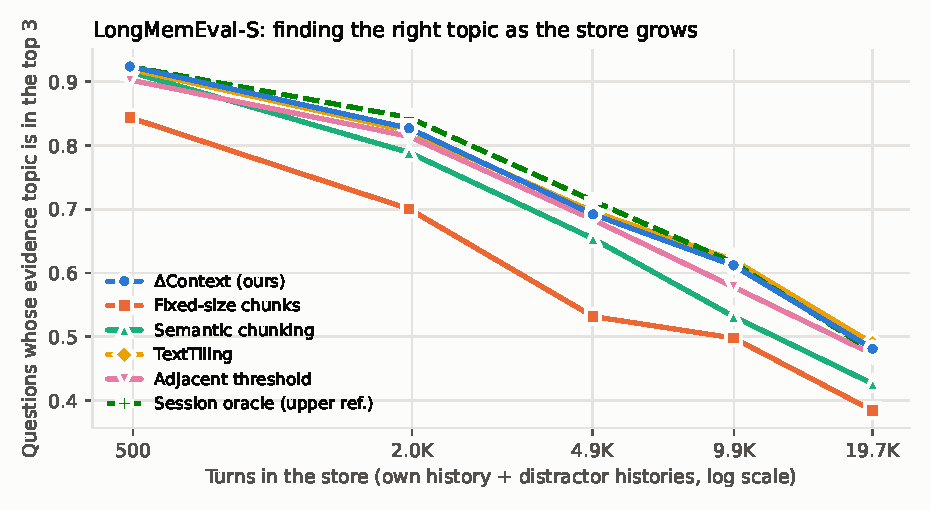
\includegraphics[width=\linewidth]{scaling.pdf}
\caption{Topic hit@3 as the store grows with distractor histories
(LongMemEval-S, 237 test-half questions). \dc{} stays on the session-oracle
curve; fixed-size chunks and semantic chunking fall behind.}
\label{fig:scaling}
\end{figure}

% =====================================================================
\section{Comparisons with Existing Works}
\label{sec:comp}

\subsection{Compared works and metrics}
\dc{} is compared with three existing families, all run on the same MiniLM
embeddings, the same splits and the same tuning protocol:
(a) \textbf{TextTiling} \cite{hearst1997texttiling}, the decoding step of CSM
and UMLF \cite{xing2021csm,xu2025umlf} and the strongest unsupervised offline
baseline available on the same encoder;
(b) \textbf{semantic chunking} \cite{langchain2024semantic}, the
percentile-threshold splitter evaluated for RAG by Lavarec and Du
\cite{lavarec2026chunking}; and (c) \textbf{full-scan turn-level dense
retrieval}, the round-level index of LongMemEval \cite{wu2025longmemeval} and
the retrieval mode of MemoryBank \cite{zhong2024memorybank}. Two common online
rules (adjacent-turn threshold, fixed-size chunks) complete the field, and
published trained segmenters are compared in Section~\ref{sec:published}.
Metrics cover segmentation (Pk, WD, $F1$, $J$), streaming (revisions, delay),
retrieval (hit@$k$, topic recall, search share) and answers (F1, EM).

\subsection{Segmentation, each method tuned per dataset}
Table~\ref{tab:seg} and Fig.~\ref{fig:segbars}(a) compare all methods.
On LongMemEval-S, \dc{} is the most accurate on every metric. Against
TextTiling, Pk is lower by 0.011 (95\% CI $[-0.014,-0.007]$) and $F1_0$ higher
by 0.020 ($[+0.015,+0.024]$), both $p<10^{-4}$. Against semantic chunking and
the adjacent threshold, Pk is lower by 0.083 and 0.064 and $F1_0$ higher by
0.158 and 0.160. It is also the best online method on all four datasets. On
SuperDialseg, offline TextTiling has a lower Pk (by 0.028, $p<10^{-4}$), while
$F1_0$ does not differ (+0.008, n.s.). On TIAGE, \dc{}, TextTiling and
semantic chunking are statistically tied. On the unseen DialSeg711,
TextTiling's SuperDialseg setting transfers better than \dc{}'s.

\begin{table*}[t]
\centering
\caption{Topic segmentation on four test sets, each method tuned on that dataset's dev split (DialSeg711: SuperDialseg setting). Cells: Pk$\downarrow$ / $F1_0\uparrow$ ($J\uparrow$). Bold: best $J$ per dataset. ``Online'': decides each boundary without later turns being able to change it.}
\label{tab:seg}
\footnotesize
\begin{tabular}{@{}lcccccc@{}}
\toprule
Method & Online & Training & LongMemEval-S & SuperDialseg & TIAGE & DialSeg711 \\
\midrule
\textbf{\dc{} v3 (ours)} & yes & none & \textbf{0.058 / 0.914 (0.928)} & 0.413 / 0.502 (0.544) & 0.427 / 0.365 (0.469) & 0.490 / 0.497 (0.503) \\
TextTiling \cite{hearst1997texttiling} & no & none & 0.069 / 0.894 (0.913) & \textbf{0.385 / 0.493 (0.554)} & 0.442 / 0.374 (0.466) & \textbf{0.401 / 0.560 (0.579)} \\
Semantic chunking \cite{langchain2024semantic} & no & none & 0.141 / 0.756 (0.808) & 0.498 / 0.399 (0.450) & \textbf{0.441 / 0.397 (0.478)} & 0.464 / 0.448 (0.492) \\
Adjacent-turn threshold & yes & none & 0.122 / 0.754 (0.816) & 0.511 / 0.408 (0.449) & 0.471 / 0.399 (0.464) & 0.499 / 0.417 (0.459) \\
Fixed-size chunks & yes & none & 0.532 / 0.170 (0.319) & 0.495 / 0.455 (0.480) & 0.544 / 0.260 (0.358) & 0.576 / 0.457 (0.441) \\
\bottomrule
\end{tabular}
\end{table*}

\begin{figure*}[t]
\centering
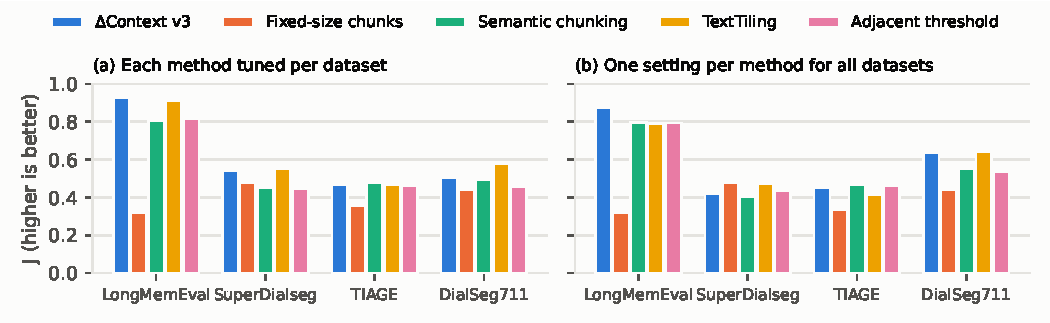
\includegraphics[width=0.92\textwidth]{segbench_bars.pdf}
\caption{Segmentation score $J$ on four test sets. (a) Each method tuned per
dataset. (b) One setting per method, chosen by mean dev $J$ over LongMemEval-S,
SuperDialseg and TIAGE and used unchanged everywhere. Significance tests for
(b) are in Table~\ref{tab:equal}.}
\label{fig:segbars}
\end{figure*}

\subsection{Segmentation under equal selection}
A deployed assistant cannot be re-tuned for each user, so we also give every
method a single setting chosen by the same rule (best mean dev $J$ over the
three dev splits). Table~\ref{tab:equal} and Fig.~\ref{fig:segbars}(b) show
the result. \dc{} beats every baseline on LongMemEval-S by at least 0.080 $J$
($p<10^{-4}$). It also beats semantic chunking, the adjacent threshold and
fixed chunks on the unseen DialSeg711, where it ties TextTiling ($-0.008$,
n.s.; \dc{} has the lower Pk, 0.283 vs.\ 0.295). On TIAGE all methods except
fixed chunks tie. On SuperDialseg, whose topics are about three turns long,
\dc{}'s single setting ($L{=}2$) trails TextTiling and fixed chunks. Notably,
TextTiling with one setting falls from 0.913 to 0.790 $J$ on LongMemEval-S,
whereas \dc{} falls only from 0.928 to 0.877, so \dc{} is the more robust
choice when one configuration must serve both long chats and short dialogues.

\begin{table}[t]
\centering
\caption{Equal selection: $\Delta J$ (\dc{} $-$ baseline) on test, one setting per method. $^{*}$Holm $p<0.05$; otherwise n.s. W/T/L: significant wins/ties/losses.}
\label{tab:equal}
\footnotesize
\setlength{\tabcolsep}{2.4pt}
\begin{tabular}{@{}lccccc@{}}
\toprule
Baseline & LongMemEval & SuperDial. & TIAGE & DialSeg711 & W/T/L \\
\midrule
TextTiling & $+0.087^{*}$ & $-0.052^{*}$ & $+0.037$ & $-0.008$ & 1/2/1 \\
Semantic chunk. & $+0.080^{*}$ & $+0.016$ & $-0.018$ & $+0.081^{*}$ & 2/2/0 \\
Adjacent thr. & $+0.083^{*}$ & $-0.014$ & $-0.013$ & $+0.099^{*}$ & 2/2/0 \\
Fixed chunks & $+0.558^{*}$ & $-0.060^{*}$ & $+0.118^{*}$ & $+0.195^{*}$ & 3/0/1 \\
\bottomrule
\end{tabular}
\end{table}

\subsection{Streaming stability}
We replayed the 250 LongMemEval-S test histories one turn at a time, re-running
the offline methods after every turn (Table~\ref{tab:storecomp}, ``Revisions''
and ``Delay''). TextTiling revises 17.0 existing boundaries per 100 new turns
(14.0 removed, 3.0 late cuts) and semantic chunking 17.6. Each revision
re-indexes stored topics and invalidates any summary or cache attached to them.
\dc{} revises none, by construction (P1), and still ends with the highest
boundary F1 (0.917 vs.\ 0.899). Its median detection delay is 4 turns
($L{+}1$), against 5 for TextTiling, which needs a full block of turns on both
sides of a gap.

\subsection{Retrieval cost and answer quality}
Table~\ref{tab:storecomp} and Fig.~\ref{fig:cost} compare the memories built
on each segmenter with full-scan retrieval. \dc{} and TextTiling give
statistically indistinguishable stores, but only \dc{}'s is built without
revisions. \dc{} leads semantic chunking on hit@1 (+0.049; not significant
after Holm correction, $p=0.013$ uncorrected on the test half) at a lower
search share, and beats 10-turn chunks by 0.23 hit@1 and 0.04 F1. The full scan
keeps the most evidence but reads every turn, and its answer F1 is within the
confidence interval of \dc{}'s. In Fig.~\ref{fig:cost}, the \dc{} curve lies
on the session-oracle curve at every top-$k$. At 19.7K turns
(Fig.~\ref{fig:scaling}), \dc{} also leads semantic chunking (hit@3 0.481 vs.\
0.426) and fixed chunks (0.384), and matches TextTiling (0.489), which performs
10\% more comparisons.

\begin{table*}[t]
\centering
\caption{Memory comparison on LongMemEval-S (budget 2,048, top-3 topics, 470 answerable questions). Pk: final segmentation in the streaming replay. ``Revisions'': boundaries changed per 100 new turns. $^{***}p<10^{-3}$, $^{*}p<0.05$ vs.\ \dc{}.}
\label{tab:storecomp}
\footnotesize
\begin{tabular}{@{}lcccccccccc@{}}
\toprule
Memory & Online & Revisions & Delay & Pk & Hit@1 & Hit@3 & Topic rec. & Searched & QA F1 & QA EM \\
\midrule
\textbf{\dc{} v3 store (ours)} & yes & \textbf{0} & 4 & \textbf{0.058} & 0.770 & \textbf{0.930} & 0.732 & 17.1\% & 0.302 & 0.206 \\
TextTiling store \cite{hearst1997texttiling} & no & 17.0 & 5 & 0.069 & \textbf{0.777} & 0.921 & 0.729 & 16.9\% & 0.296 & 0.200 \\
Semantic chunking store \cite{langchain2024semantic,lavarec2026chunking} & no & 17.6 & 1$^{\dagger}$ & 0.141 & 0.721 & 0.904 & 0.704 & 18.4\% & 0.284 & 0.194 \\
Adjacent-threshold store & yes & 0 & 1 & 0.122 & 0.736 & 0.902 & 0.711 & 20.1\% & -- & -- \\
Fixed-size chunks (10 turns) & yes & 0 & 1 & 0.500 & 0.543$^{***}$ & 0.813$^{***}$ & 0.601$^{***}$ & 16.2\% & 0.263$^{*}$ & 0.187 \\
Full scan, turn level \cite{wu2025longmemeval,zhong2024memorybank} & yes & -- & -- & -- & -- & -- & \textbf{0.774}$^{***}$ & 100\% & \textbf{0.311} & \textbf{0.217} \\
\midrule
Session oracle (reference) & -- & -- & -- & 0 & 0.785 & 0.926 & 0.733 & 16.5\% & 0.298 & 0.202 \\
\bottomrule
\multicolumn{11}{@{}l}{\scriptsize $^{\dagger}$Median; semantic chunking's mean delay is 14.5 turns because many boundaries appear only after later percentile shifts.}
\end{tabular}
\end{table*}

\begin{figure}[t]
\centering
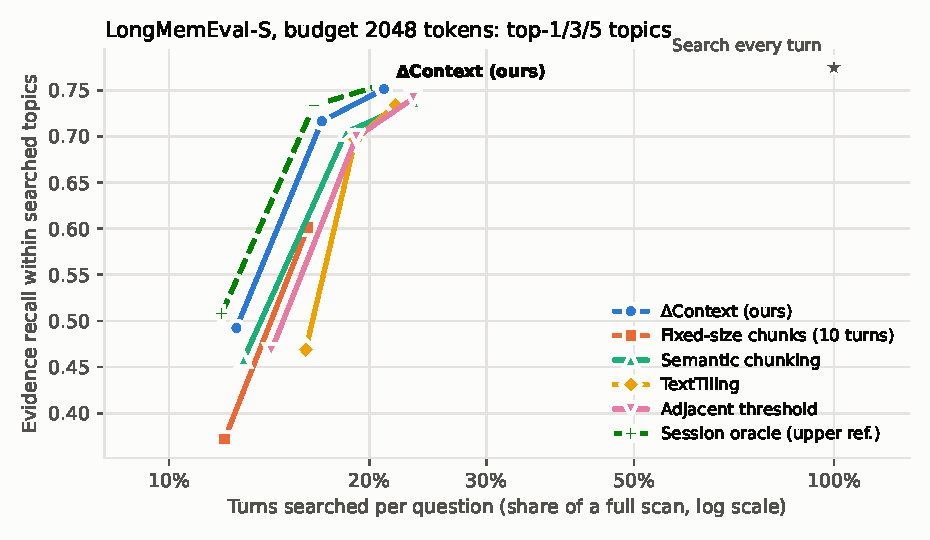
\includegraphics[width=\linewidth]{cost_recall.pdf}
\caption{Evidence recall against the share of turns searched (top-1/3/5
topics; LongMemEval-S, 2,048-token budget). The \dc{} store reaches the
session-oracle trade-off; a full scan reads every turn.}
\label{fig:cost}
\end{figure}

\subsection{Comparison with published dialogue segmenters}
\label{sec:published}
Table~\ref{tab:published} places \dc{} next to published unsupervised
segmenters, as reported by Xu et al.\ \cite{xu2025umlf}. These methods train
neural scorers or encoders on in-domain dialogues and decode offline. \dc{}
uses a 22M-parameter off-the-shelf encoder, no training and online decisions.
On TIAGE, the single \dc{} setting scores 61.2 (1$-$Pk), above the 59.3 that
UMLF reports. On DialSeg711 it scores 71.7, above TeT+CLS
\cite{xu2021dialseg711} but 4--14 points below CSM, DialSTART and UMLF. The
numbers are indicative only: encoders, training data and Pk window conventions
differ, and the TIAGE dev split took part in choosing the single setting.

\begin{table}[t]
\centering
\caption{1$-$Pk / 1$-$WD (\%, higher is better). Published rows from \cite{xu2025umlf}; different encoders and training, so indicative only.}
\label{tab:published}
\footnotesize
\setlength{\tabcolsep}{3pt}
\begin{tabular}{@{}lccc@{}}
\toprule
Method & Trained / online & TIAGE & DialSeg711 \\
\midrule
TeT+CLS \cite{xu2021dialseg711} & no / no & 52.7 / 48.6 & 59.5 / 56.9 \\
CSM \cite{xing2021csm} & yes / no & 52.8 / 49.1 & 75.7 / 73.7 \\
DialSTART \cite{gao2023dialstart} & yes / no & 55.7 / 50.2 & 82.1 / 80.2 \\
UMLF \cite{xu2025umlf} & yes / no & 59.3 / 55.6 & \textbf{85.9 / 84.2} \\
\midrule
TextTiling, MiniLM (our run) & no / no & 56.1 / 54.8 & 70.5 / 67.8 \\
\textbf{\dc{} v3, one setting} & no / \textbf{yes} & \textbf{61.2 / 60.0} & 71.7 / 69.1 \\
\bottomrule
\end{tabular}
\end{table}

\subsection{Summary of the comparison}
On long chat histories, the setting a conversational memory faces, \dc{} beats
offline TextTiling under both tuning protocols and every online rule. It is the
only accurate method that never revises a boundary, so its segments can serve
as a persistent index, and its store matches a true-session store while
answering as well as a full scan at about a sixth of the cost. Its limits: on
short dialogue benchmarks it ties offline TextTiling (TIAGE, DialSeg711) or
trails it (SuperDialseg); trained offline segmenters are more accurate on
DialSeg711; and a full scan keeps 4 points more evidence. Delayed commitment
was introduced after the immediate-decision v2 lost on the dialogue
benchmarks, which is why all comparisons use dev-only tuning and one test pass.

% =====================================================================
\section{Conclusion}
\label{sec:concl}
This paper presented \dc{}, which stores a growing chat as topic segments
found online and retrieves by topic first. Its novelty is delayed commitment:
each gap is judged against the turns that follow it and committed only at a
local maximum, so boundaries are final, arrive after a constant delay and need
no training. On long chat histories \dc{} was the most accurate segmenter
compared, including offline TextTiling, while revising no boundary where
offline methods revised about seventeen per hundred turns. The resulting store
matched a true-session store up to twenty thousand turns and answered as well
as scanning every turn while searching about a sixth of them. On short dialogue
benchmarks it was the best online method but tied or trailed the best offline
one. Future work will adapt the look-ahead to topic length within a
conversation, and attach compact per-topic summaries and hierarchical topic
links so that very large stores can be searched in one step.

% =====================================================================
\begin{thebibliography}{99}

\bibitem{ni2023survey}
J.~Ni, T.~Young, V.~Pandelea, F.~Xue, and E.~Cambria, ``Recent advances in deep learning based dialogue systems: A systematic survey,'' \emph{Artificial Intelligence Review}, vol.~56, no.~4, pp.~3055--3155, 2023, doi: 10.1007/s10462-022-10248-8.

\bibitem{wang2024agents}
L.~Wang, C.~Ma, X.~Feng, Z.~Zhang, H.~Yang, J.~Zhang, Z.~Chen, J.~Tang, X.~Chen, Y.~Lin, W.~X. Zhao, and Z.~Wei, ``A survey on large language model based autonomous agents,'' \emph{Frontiers of Computer Science}, vol.~18, no.~6, Art.~no.~186345, 2024, doi: 10.1007/s11704-024-40231-1.

\bibitem{zhang2025memory}
Z.~Zhang, Q.~Dai, X.~Bo, C.~Ma, R.~Li, X.~Chen, J.~Zhu, Z.~Dong, and J.-R. Wen, ``A survey on the memory mechanism of large language model-based agents,'' \emph{ACM Transactions on Information Systems}, vol.~43, no.~6, pp.~1--47, 2025, doi: 10.1145/3748302.

\bibitem{tay2022efficient}
Y.~Tay, M.~Dehghani, D.~Bahri, and D.~Metzler, ``Efficient transformers: A survey,'' \emph{ACM Computing Surveys}, vol.~55, no.~6, pp.~1--28, 2022, doi: 10.1145/3530811.

\bibitem{liu2024lost}
N.~F. Liu, K.~Lin, J.~Hewitt, A.~Paranjape, M.~Bevilacqua, F.~Petroni, and P.~Liang, ``Lost in the middle: How language models use long contexts,'' \emph{Transactions of the Association for Computational Linguistics}, vol.~12, pp.~157--173, 2024, doi: 10.1162/tacl\_a\_00638.

\bibitem{huang2025hallucination}
L.~Huang, W.~Yu, W.~Ma, W.~Zhong, Z.~Feng, H.~Wang, Q.~Chen, W.~Peng, X.~Feng, B.~Qin, and T.~Liu, ``A survey on hallucination in large language models: Principles, taxonomy, challenges, and open questions,'' \emph{ACM Transactions on Information Systems}, vol.~43, no.~2, pp.~1--55, 2025, doi: 10.1145/3703155.

\bibitem{wu2026rag}
S.~Wu, Y.~Xiong, Y.~Cui, H.~Wu, C.~Chen, Y.~Yuan, L.~Huang, X.~Liu, T.-W. Kuo, N.~Guan, and C.~J. Xue, ``Retrieval-augmented generation for natural language processing: A survey,'' \emph{Artificial Intelligence Review}, vol.~59, no.~9, Art.~no.~192, 2026, doi: 10.1007/s10462-026-11605-7.

\bibitem{zhao2024dense}
W.~X. Zhao, J.~Liu, R.~Ren, and J.-R. Wen, ``Dense text retrieval based on pretrained language models: A survey,'' \emph{ACM Transactions on Information Systems}, vol.~42, no.~4, pp.~1--60, 2024, doi: 10.1145/3637870.

\bibitem{pan2024vectordb}
J.~J. Pan, J.~Wang, and G.~Li, ``Survey of vector database management systems,'' \emph{The VLDB Journal}, vol.~33, no.~5, pp.~1591--1615, 2024, doi: 10.1007/s00778-024-00864-x.

\bibitem{wang2025recursive}
Q.~Wang, Y.~Fu, Y.~Cao, S.~Wang, Z.~Tian, and L.~Ding, ``Recursively summarizing enables long-term dialogue memory in large language models,'' \emph{Neurocomputing}, vol.~639, Art.~no.~130193, 2025, doi: 10.1016/j.neucom.2025.130193.

\bibitem{zhong2024memorybank}
W.~Zhong, L.~Guo, Q.~Gao, H.~Ye, and Y.~Wang, ``MemoryBank: Enhancing large language models with long-term memory,'' in \emph{Proc. AAAI Conf. Artificial Intelligence}, vol.~38, no.~17, pp.~19724--19731, 2024, doi: 10.1609/aaai.v38i17.29946.

\bibitem{packer2023memgpt}
C.~Packer, S.~Wooders, K.~Lin, V.~Fang, S.~G. Patil, I.~Stoica, and J.~E. Gonzalez, ``MemGPT: Towards LLMs as operating systems,'' arXiv:2310.08560, 2023.

\bibitem{wu2025longmemeval}
D.~Wu, H.~Wang, W.~Yu, Y.~Zhang, K.-W. Chang, and D.~Yu, ``LongMemEval: Benchmarking chat assistants on long-term interactive memory,'' in \emph{Proc. Int. Conf. Learning Representations (ICLR)}, 2025.

\bibitem{ma2024topicaware}
X.~Ma, Y.~Xu, H.~Zhao, and Z.~Zhang, ``Multi-turn dialogue comprehension from a topic-aware perspective,'' \emph{Neurocomputing}, vol.~578, Art.~no.~127385, 2024, doi: 10.1016/j.neucom.2024.127385.

\bibitem{sun2022hierarchical}
X.~Sun and B.~Ding, ``Neural network with hierarchical attention mechanism for contextual topic dialogue generation,'' \emph{IEEE Access}, vol.~10, pp.~4628--4639, 2022, doi: 10.1109/ACCESS.2022.3140820.

\bibitem{xu2025umlf}
J.~Xu, F.~Jiang, A.~Gao, L.~F. D'Haro, and H.~Li, ``Unsupervised mutual learning of discourse parsing and topic segmentation in dialogue,'' \emph{IEEE Transactions on Audio, Speech and Language Processing}, vol.~33, pp.~4667--4681, 2025, doi: 10.1109/TASLPRO.2025.3623884.

\bibitem{lavarec2026chunking}
E.~Lavarec and Y.~Du, ``Evaluating document chunking approaches for retrieval augmented generation in editorial content,'' \emph{IAES International Journal of Artificial Intelligence}, vol.~15, no.~2, pp.~1909--1918, 2026, doi: 10.11591/ijai.v15.i2.pp1909-1918.

\bibitem{hearst1997texttiling}
M.~A. Hearst, ``TextTiling: Segmenting text into multi-paragraph subtopic passages,'' \emph{Computational Linguistics}, vol.~23, no.~1, pp.~33--64, 1997.

\bibitem{xing2021csm}
L.~Xing and G.~Carenini, ``Improving unsupervised dialogue topic segmentation with utterance-pair coherence scoring,'' in \emph{Proc. 22nd Annu. Meeting Special Interest Group on Discourse and Dialogue (SIGDIAL)}, 2021, pp.~167--177, doi: 10.18653/v1/2021.sigdial-1.18.

\bibitem{gao2023dialstart}
H.~Gao, R.~Wang, T.-E. Lin, Y.~Wu, M.~Yang, F.~Huang, and Y.~Li, ``Unsupervised dialogue topic segmentation with topic-aware contrastive learning,'' in \emph{Proc. 46th Int. ACM SIGIR Conf. Research and Development in Information Retrieval}, 2023, pp.~2481--2485, doi: 10.1145/3539618.3592081.

\bibitem{jiang2023superdialseg}
J.~Jiang, C.~Dong, S.~Kurohashi, and A.~Aizawa, ``SuperDialseg: A large-scale dataset for supervised dialogue segmentation,'' in \emph{Proc. Conf. Empirical Methods in Natural Language Processing (EMNLP)}, 2023, pp.~4086--4101, doi: 10.18653/v1/2023.emnlp-main.249.

\bibitem{nouar2026boundary}
F.~Nouar and H.~Belhadef, ``Boundary-centered explainability for dialogue topic segmentation,'' \emph{Electronics}, vol.~15, no.~17, Art.~no.~3998, 2026, doi: 10.3390/electronics15173998.

\bibitem{langchain2024semantic}
LangChain, ``SemanticChunker (langchain\_experimental.text\_splitter),'' 2024. [Online]. Available: \url{https://python.langchain.com}

\bibitem{veena2023agroner}
G.~Veena, V.~Kanjirangat, and D.~Gupta, ``AGRONER: An unsupervised agriculture named entity recognition using weighted distributional semantic model,'' \emph{Expert Systems with Applications}, vol.~229, Art.~no.~120440, 2023, doi: 10.1016/j.eswa.2023.120440.

\bibitem{veena2023relation}
G.~Veena, D.~Gupta, and V.~Kanjirangat, ``Semi-supervised bootstrapped syntax-semantics-based approach for agriculture relation extraction for knowledge graph creation and reasoning,'' \emph{IEEE Access}, vol.~11, pp.~138375--138398, 2023, doi: 10.1109/ACCESS.2023.3339552.

\bibitem{venugopalan2022guidedlda}
M.~Venugopalan and D.~Gupta, ``An enhanced guided LDA model augmented with BERT based semantic strength for aspect term extraction in sentiment analysis,'' \emph{Knowledge-Based Systems}, vol.~246, Art.~no.~108668, 2022, doi: 10.1016/j.knosys.2022.108668.

\bibitem{gurusamy2023summarization}
B.~M. Gurusamy, P.~K. Rengarajan, and P.~Srinivasan, ``A hybrid approach for text summarization using semantic latent Dirichlet allocation and sentence concept mapping with transformer,'' \emph{International Journal of Electrical and Computer Engineering}, vol.~13, no.~6, pp.~6663--6672, 2023, doi: 10.11591/ijece.v13i6.pp6663-6672.

\bibitem{reimers2019sbert}
N.~Reimers and I.~Gurevych, ``Sentence-BERT: Sentence embeddings using Siamese BERT-networks,'' in \emph{Proc. Conf. Empirical Methods in Natural Language Processing and Int. Joint Conf. Natural Language Processing (EMNLP-IJCNLP)}, 2019, pp.~3980--3990, doi: 10.18653/v1/D19-1410.

\bibitem{qwen2024qwen25}
Qwen Team, ``Qwen2.5 technical report,'' arXiv:2412.15115, 2024.

\bibitem{beeferman1999statistical}
D.~Beeferman, A.~Berger, and J.~Lafferty, ``Statistical models for text segmentation,'' \emph{Machine Learning}, vol.~34, pp.~177--210, 1999.

\bibitem{pevzner2002critique}
L.~Pevzner and M.~A. Hearst, ``A critique and improvement of an evaluation metric for text segmentation,'' \emph{Computational Linguistics}, vol.~28, no.~1, pp.~19--36, 2002.

\bibitem{holm1979simple}
S.~Holm, ``A simple sequentially rejective multiple test procedure,'' \emph{Scandinavian Journal of Statistics}, vol.~6, no.~2, pp.~65--70, 1979.

\bibitem{xie2021tiage}
H.~Xie, Z.~Liu, C.~Xiong, Z.~Liu, and A.~Copestake, ``TIAGE: A benchmark for topic-shift aware dialog modeling,'' in \emph{Findings of the Association for Computational Linguistics: EMNLP 2021}, 2021, pp.~1684--1690, doi: 10.18653/v1/2021.findings-emnlp.145.

\bibitem{xu2021dialseg711}
Y.~Xu, H.~Zhao, and Z.~Zhang, ``Topic-aware multi-turn dialogue modeling,'' in \emph{Proc. AAAI Conf. Artificial Intelligence}, vol.~35, no.~16, pp.~14176--14184, 2021, doi: 10.1609/aaai.v35i16.17668.

\end{thebibliography}

\end{document}
